\section{Appendix for "\ours: Unlocking the Power of Code Instruction Tuning by Simply Merging Upcycled Mixture-of-Experts"}
\label{sec:appendix}

\subsection{Hyperparameter Settings}\label{sec:hyperparameter}
We use a batch size of 64 and a learning rare of 5e-5 with a linear scheduler to fine-tune \textbf{\oursmoe} for 4 epochs with 500 warmup steps, following the implementation of previous work~\cite{wei2023magicoder}. We further use a batch size of 64, a shared expert rate $\lambda$ of 0.75, and a learning rare of 1e-5 with a linear schedule to fine-tune the learnable mixing coefficients for each of the experts in the instruction-tuned \textbf{\oursmoe} on the instruction dataset for 1 epoch with 125 warmup steps. Detailedly, we use Softmax to keep the sum of the mixing coefficients of the other 7 normal experts as 0.25. For \textbf{\baselineds} and \textbf{\ewads}, we use the same hyperparameter setting as \ours, where the batch size is 64 and the learning rate is 5e-5 with a linear scheduler. Because \ours is trained for 4 epochs during upcycling and 1 epoch during merging, for a fair comparison, we train \baselineds and \ewads for 5 (= 4 + 1) epochs with 625 warmup steps.

\subsection{Implementation details of \ewa}\label{sec:ewa_details}
Because \ewa~\cite{huang2023experts} does not release their implementation, we implemented \ewa by ourselves, including constant schedule and linear schedule. We use a share rate $\beta$ of 0.3, following the original setting of \ewa. While \ewa with the constant schedule achieves reasonable performance in our evaluation, the training loss of \ewa with the linear schedule becomes very unstable, as is shown in Figure \ref{fig:loss_ewa}, and thus cannot achieve reasonable performance. As a result, we report the results of \ewa with the constant schedule in Section \ref{sec:experiment}.

\begin{figure}[ht]
\centering
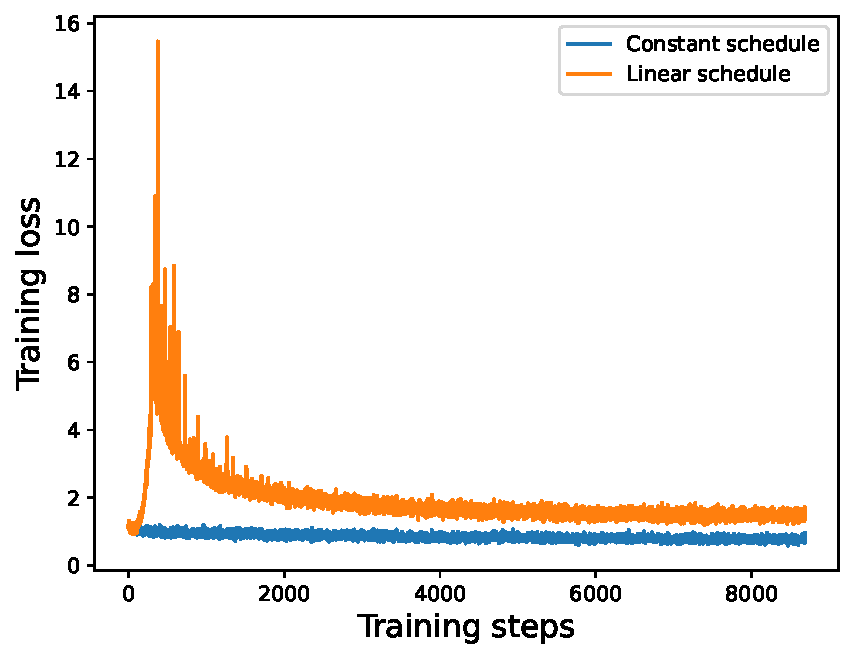
\includegraphics[width=1.0\linewidth]{assets/loss_ewa.pdf}
\caption{Training loss curve of \ewa with constant schedule and linear schedule.}
\label{fig:loss_ewa}
\end{figure}


\subsection{Details of \humaneval and \mbpp}\label{sec:benchmarks}
In these benchmarks, each task consists of a task description in English, which is sent to \llm{s} as the prompt, and \llm{s} are expected to generate the corresponding code to satisfy the requirements in the description. While these benchmarks provide a handful of test cases to validate the correctness of the generated code, these tests are often insufficient for more rigorous evaluation. As such, \humanevalp and \mbppp proposed by \evalplus~\cite{evalplus} are usually used to evaluate the correctness of the generated code, which provides 80×/35× more tests compared with the original benchmarks.

\subsection{Statistical Significance Analysis}\label{sec:statistic}
\begin{table}[t]
\centering
\begin{tabular}{@{}lrr@{}}
\toprule
Model                         & \multicolumn{1}{c}{HumanEval} & \multicolumn{1}{c}{HumanEval+} \\ \midrule
\baselineds                      & 61.6                          & 57.2                           \\
\ewads & 62.7                          & 58.8                           \\
\oursmerge                      & \textbf{64.5}                 & \textbf{60.9}                  \\ \bottomrule
\end{tabular}
\caption{\label{tab:discussion-stat-mean}
Average pass@1 results of 200 experiments on \humaneval{}~(+) computed with sampling. \ours clearly outperforms both \ewads and \baselineds.
}
\end{table}

\begin{table}[t]
\centering
\begin{tabular}{@{}lrr@{}}
\toprule
Model            & \multicolumn{1}{c}{HumanEval} & \multicolumn{1}{c}{HumanEval+} \\ \midrule
\scalebox{0.9}{\oursmerge vs. \ewads} & 2.6e-18                       & 8.0e-23                        \\
\scalebox{0.9}{\oursmerge vs. \baselineds} & 9.6e-30                       & 3.7e-33                        \\ \bottomrule
\end{tabular}
\caption{\label{tab:discussion-stat-p}
$p$-values for \oursmerge vs. \ewads and \oursmerge vs. \baselineds in 200 experiments on \humaneval{}~(+) computed with sampling. Results show that improvements brought by \ours are statistically significant.
}
\end{table}


In this section, we show that improvements brought by \ours are statistically significant. In our main experiments, we follow prior works~\cite{wei2023magicoder, lozhkov2024starcoder} to conduct experiments on \humaneval{}~(+) using greedy decoding. To demonstrate the statistical significance of our improvements, we change our setting from greedy decoding to sampling. In detail, to conduct one experiment on \humaneval{}~(+), the model will sample one solution for each problem in \humaneval{}~(+) with top $p$ = 0.95 and temperature = 0.8, which is the same setting used in prior works~\cite{evalplus, chen2021evaluating}.

Following prior work~\cite{evalplus}, we repeat this experiment 200 times for three techniques: \oursmerge, \ewads, and \baselineds. \ewads is included because it is the best-performing baseline in our main experiment. We first compute their average pass@1 performance in these 200 experiments. As is shown in Table \ref{tab:discussion-stat-mean}, \oursmerge outperforms both \ewads and \baselineds clearly.

Furthermore, we use the Wilcoxon signed-rank test~\cite{Wilcoxon1945IndividualCB, dror-etal-2018-hitchhikers}, a widely used statistical test, to check if the improvements brought by \ours are statistically significant. As shown in Table \ref{tab:discussion-stat-p}, the $p$-values for both \oursmerge vs. \ewads and \oursmerge vs. \baselineds are much smaller than both 0.0025 (the significance level recommended for NLP work by~\cite{sogaard-etal-2014-whats}) and 0.05 (the most common significance level), demonstrating the statistical significance of the improvements brought by \ours.

\subsection{Analysis on Expert Specialization}\label{sec:expert_analysis}
\begin{figure*}[ht]
\centering
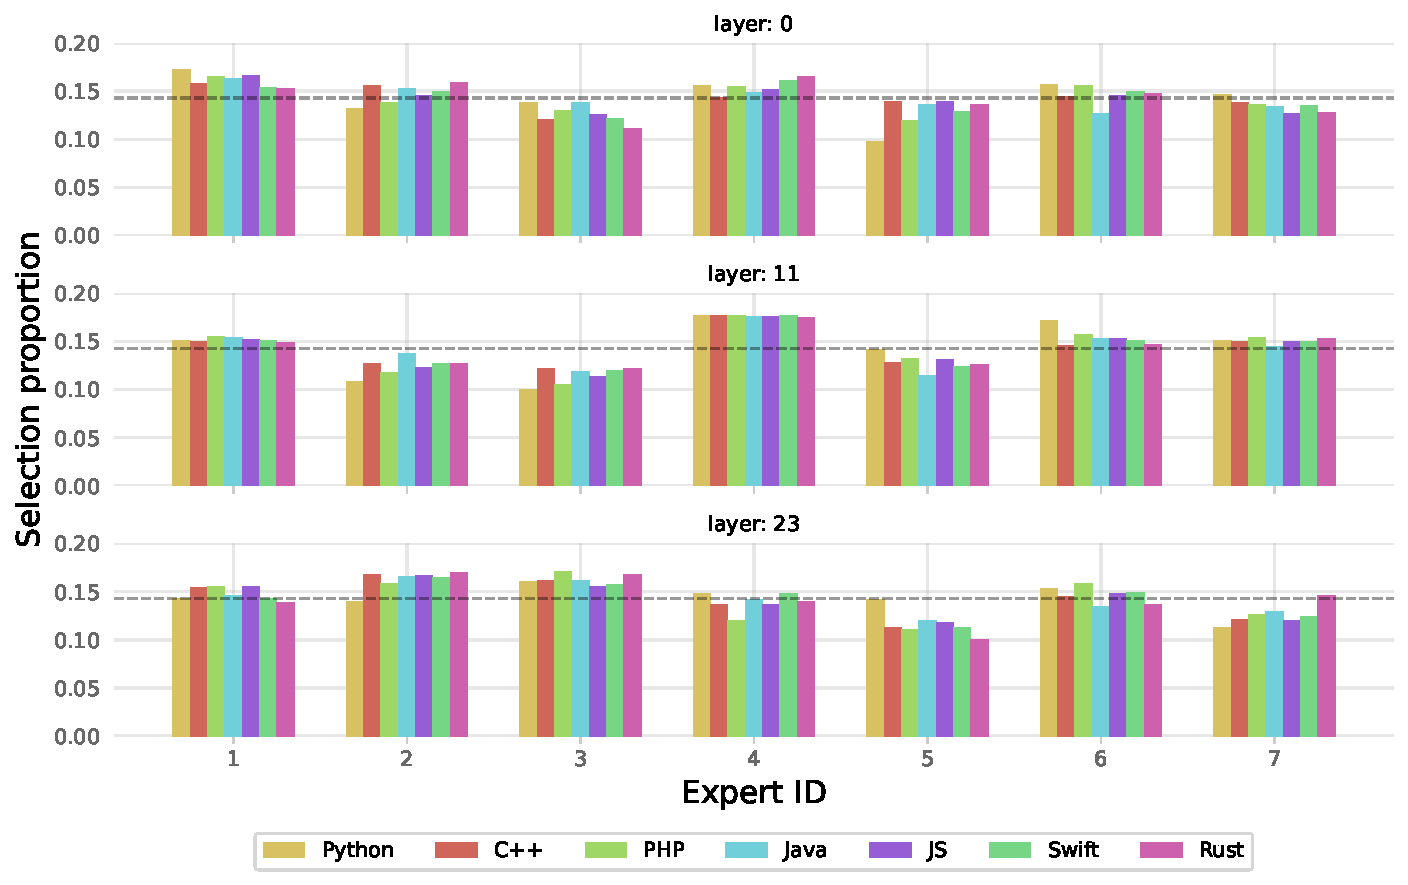
\includegraphics[width=1.0\linewidth]{assets/analysis.pdf}
\caption{Proportion of tokens assigned to each expert on different programming languages from \multiple (including Python) for layers 0, 11, and 23. The shared expert 0 is excluded from the chart because all the tokens are always assigned to it. The gray vertical line marks $\frac{1}{7}$, which is the proportion expected with the uniform sampling.}
\label{fig:analysis}
\end{figure*}

Inspired by recent works~\cite{jiang2024mixtral, xue2024openmoe}, we analyze whether each expert in \oursmoe has different specializations in different programming languages
by visualizing the routing decision of the tokens from different programming languages in the \multiple benchmark (including Python). For the \multiple benchmark, we collect the routing decision when conducting experiments in Section \ref{sec:multiple}. For Python, we collect the routing decision by reruning \humaneval experiment following the same setting as Section \ref{sec:multiple}. Following Mixtral~\cite{jiang2024mixtral}, we get the visualization results from layers 0, 11, and 23 in \oursmoe, where layer 0 and layer 23 are the first and the last layers of \oursmoe. As is shown in Figure \ref{fig:analysis}, we do not observe obvious
patterns in the assignment of experts based on the programming language, which is in line with the observation reported by recent works~\cite{jiang2024mixtral, xue2024openmoe}. 
1681
\subsection{Training Settings for \stablecoder 3B}\label{sec:stable_setting}
We use \evolcode as the training dataset. Since \stablecoder 3B is the base model, we upcycle a new \moe model from the base model, namely \textbf{\stablemoe}. Due to limited computational resources, we construct \stablemoe with 4 experts in one expert layer, where the top 2 experts are activated for each token, including one shared expert. Consequently, the size of \stablemoe can be described as 4$\times$3B. We use a batch size of 64 and a learning rate of 5e-5 with a linear scheduler to fine-tune \stablemoe for 4 epochs with 500 warmup steps. Similar to \oursmerge, we obtain \textbf{\stablemerge} by learning mixing coefficients to merge \moe layers inside \stablemoe as normal FFN layers, which is fine-tuned with a batch size of 64, a shared expert rate $\lambda$ of 0.85, and a learning rate of 1e-5 with a linear schedule for 1 epoch with 125 warmup steps. Our baseline model, namely \textbf{\baselinestable}, is fine-tuned for 5 (= 4 + 1) epochs with a batch size of 64, a learning rate of 5e-5, and 625 warmup steps for a fair comparison.

\subsection{Training Settings for \tinyllama 1.1B}\label{sec:tinyllama_setting}
Using \tinyllama 1.1B as the base model, we upcycle a new \moe model, namely \textbf{\tinyllamamoe}, from the base model. Following the setting for \oursmoe, we construct \tinyllamamoe with 8 experts in one expert layer, where the top 6 experts are activated for each token, including one shared expert. As such, the number of parameters for \tinyllamamoe can be written as 8$\times$1.1B. We use a batch size of 64 and a learning rate of 5e-5 with a linear scheduler to fine-tune \tinyllamamoe for 4 epochs with 240 warmup steps. To obtain \textbf{\tinyllamamerge}, we learn mixing coefficients to merge \moe layers inside \tinyllamamoe by fine-tuning them with a batch size of 64, a shared expert rate $\lambda$ of 0.85, and a learning rate of 2e-5 with a linear schedule for 1 epoch with 60 warmup steps. For a fair comparison, we fine-tune a baseline model \textbf{\baselinetinyllama} for 5 (= 4 + 1) epochs with a batch size of 64, a learning rate of 5e-5, and 300 warmup steps.

\subsection{Theoratical Explanation Details}\label{sec:theoratical_analysis}
We consider a simplified variant of \ours as below:
\begin{itemize}[leftmargin=1em]
\setlength{\parskip}{2pt}
\setlength\itemsep{0pt}
\item The original dense model is a one-layer transformer model, which contains one attention layer connected with one feed-forward network (FFN) layer. As such, the upcycled \moe model is also a one-layer transformer model, containing one attention layer connected with an \moe layer.
\item The upcycled \moe model only has two experts ($\textbf{e}_1$ and $\textbf{e}_2$), both of which are always selected for processing the input tokens.
\item The router in the \moe model assigns constant weights to each expert, regardless of the input token. Consequently, the output of the \moe layer for the $t$-th token $\textbf{h}_t$ can be represented as $(1-\alpha) \textbf{e}_1(\textbf{u}_t) + \alpha \textbf{e}_2(\textbf{u}_t)$, where $1-\alpha$ is the router weight assigned to $\textbf{e}_1$, $\alpha$ is the router weight assigned to $\textbf{e}_2$, and $\textbf{u}_t$ is the input of the \moe layer for the $t$-th token.
\item We simplify the process of merging the \moe model back to a dense model as $\textbf{W}_{\textbf{e}_{\alpha}} = (1-\alpha) \textbf{W}_{\textbf{e}_1} + \alpha \textbf{W}_{\textbf{e}_2}$, where $\textbf{W}_\textbf{e}$ refers to the weight of $\textbf{e}$ and $\textbf{e}_{\alpha}$ refers to the weight of the FFN in the merged dense model.
\end{itemize}

In this simplified scenario, if we denote $f(x;\theta)$ as the output of the model $\theta$ for the input $x$, the output of this simplified MoE model for input token $x$ can be represented as $f(x;\theta_{\textbf{MoE}})$. Interestingly, if we define two new dense models $\theta_1$ and $\theta_2$, where $\theta_1$ and $\theta_2$ use the same attention layer as this \moe model while using $\textbf{e}_1$ and $\textbf{e}_2$ as the FFN layer separately, $f(x;\theta_{\textbf{MoE}})$ can be represented as $(1-\alpha) f(x;\theta_1) + \alpha f(x;\theta_2)$! Consequently, the computation process of this simplified \moe model can be viewed as ensembling the outputs of two dense models $\theta_1$ and $\theta_2$. Meanwhile, the process of merging the upcycled \moe model back to a dense model in this simplified \ours can be represented as $\theta_{\alpha} = (1-\alpha) \theta_1 + \alpha \theta_2$, which is the merging of the same two dense models $\theta_1$ and $\theta_2$.
